\chapter{Závěr: Zhodnocení}

\section{Jednoduché škálování}
App Engine nám umožňuje psát jednoduše škálovatelné aplikace a poskytuje nám k tomuto účelu zajímavou platformu pro jednoduchý vývoj a nasazení aplikací (viz obrázek \ref{fig:app-engine-dashboard}). Možnost jednoduché škálovatelnosti ale přináší do vývoje některá omezení a rozdílné vývojářské postupy. App Engine motivuje pro využití svých služeb velmi zajímavým business modelem, kde malé a málo využívané aplikace nemusí platit nic a platba za hosting je nutná až po překročení vysokých kvót. Toto je velmi zajímavá možnost pro začínající aplikace, takzvané \emph{start-upy}, kde můžeme spustit projekt ihned a výdaje spojené s hostingem přijdou, až aplikace začne prosperovat.

\begin{figure}[h]
\begin{center}
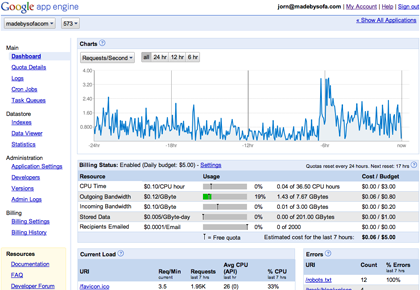
\includegraphics[width=5.7in]{figures/app-engine-dashboard.png}
\caption[App Engine Dashboard]{App Engine Dashboard 
(Zdroj: http://www.madebysofa.com/blog/appengine-hosting/)}
\label{fig:app-engine-dashboard}
\end{center}
\end{figure}

\section{Zhodnocení porovnání Datastore API, JPA, JDO}
Jako výsledek této bakalářské práce vzniklo několik aplikací. Většina z nich byly jen testovací prototypy na ověření některé z funkčností, anebo pro vyzkoušení práce se službami, které App Engine nabízí. Nejzajímavějšími z nich byly tři aplikace TodoList, pro tři různé využití možnosti práce s uložištěm: Datastore API, JPA a JDO. Tyto aplikace sloužily k porovnání rychlosti každého z těchto přístupů. Nejrychlejším z těchto přístupů byl dle očekávání Datastore API, který je připraven právě pro práci s Datastore, nevýhodou je složitější práce než~s~JPA a~JDO. Dalším důležitým poznatkem je, že uložiště na App Engine je optimalizované pro čtení, takže je výběr dat několikanásobně rychlejší než vkládání, úprava a mazání dat.

Do budoucna by se dal otestovat výběr více závislých entit z uložiště s různými typy relací (\emph{one-to-one}, \emph{one-to-many} a \emph{many-to-many}). Každý ze způsobů práce s uložištěm může využívat jiný typ propojení - muselo by se zařídít, aby byly testy spravedlivé. Všechny typy spojení by musely být v Datastore uloženy stejně.

\section{Zhodnocení porovnání testů zátěže}
Největší a nejpřínosnější aplikací je Content Management System využívající framework Slim3, který je optimalizovaný přesně pro použití na App Engine. Tato aplikace je nejrozsáhlejší a bez problému může být nasazena pro jednoduché stránky. Hlavním přínosem této aplikace bylo vyzkoušet reálnou aplikaci s vazbami mezi entitami. Pro tuto aplikaci bylo velmi výhodné použití frameworku, který urychlil vývoj a pomohl usnadnit některé části programu, například optimistické zamykání. Navíc nám tento framework dává dost volnosti, takže z něj můžeme například použít jen část pro práci s uložištěm. 

Tato aplikace byla použita na testování vysoké zátěže na rozsáhlejší a plnohodnotnou aplikaci. Cílem testu bylo zjistit, jak se bude App Engine chovat a jak kvalitní bude možnost rozložení zátěže. Na aplikaci bylo posláno velké množství požadavků a byl měřen celkový čas zpracování požadavků a rychlost odpovědi aplikace.
App Engine si sám podle zatížení aplikace rozhodl, kolik instancí aplikace má být nahráno, aby byly všechny požadavky zpracovány a zátěž byla rovnoměrně rozložena. O toto všechno se stará App Engine sám, navíc rozhodne na které z datacenter aplikaci nahraje. Kvóty touto zátěží byly ovlivněny jen minimálně. Jedině u procesorového času byla vidět větší spotřeba, ale stále zde byly rezervy. 

\section{Osobní přínos}
Největším přínosem pro mne osobně, bylo napsání větší aplikace pro App Engine. Dříve jsem zkoušel jen některé jednoduché aplikace pro vlastní potřebu. Většina z nich sloužila jen pro~demonstraci určitého API. Nyní mám praktické zkušenosti s větší aplikací a~myslím, že~jsem dokázal proniknout do fungování App Engine a dobře znám jeho výhody a nevýhody. Troufnul bych si nyní i na rozsáhlejší aplikaci s reálnou zátěží a plánuji do~budoucna takovouto aplikaci napsat. Zajímavá se mi jeví možnost naprogramovat aplikaci pro sociální sítě, kde~se zajímavé projekty rozšíří velmi rychle a App Engine je tedy vhodným kandidátem, v~opačném případě pokud aplikace nebude pro uživatele zajímavá, budou náklady na hosting nulové.

Kromě práce s App Engine jsem se při vytváření této bakalářské práce naučil efektivně využívat verzovací systém Git\footnote{Git --- http://git-scm.com/} a všechny zdrojové kódy jsou tak k dispozici na verzovacím hostingu Github na adrese: \verb|http://github.com/jskvara|. Dále jsem pro publikování výsledků práce využíval hosting projeků na Google code\footnote{Google code --- http://code.google.com/}, kde je možnost publikovat své výsledky, zdrojové kódy, aplikace ke stažení, dokumentaci projektu ve formátu wiki\footnote{Wiki formát je určen pro publikaci převážně HTML (HyperText Markup Language) obsahu generovaného běžnými uživateli, kde je syntaxe pro uživatele přívětivější} a další. Při samotném vytváření textu bakalářské práce, jsem se seznámil se nástrojem \LaTeX, který slouží k profesionální sazbě a tisku dokumentů, což pro mne bylo velmi zajímavé a určitě tento formát v budoucnu použiji znovu.